\section{Extensions}
\label{sec:extensions}
  
\subsection{Beta Distribution Bag-of-words}
\label{sec:bow_beta}
The bag-of-words model described in Section \ref{sec:bag_of_words} has some substantial issues regarding the probability estimates $p_w^a$. Most notably is its bias towards words which occur only very few times, and only with a single author.

A good example is the word "marker". In the training set Lovecraft uses it exactly once, but both Shelly and Poe don't use it at all. Is it fair for this to be considered a "signature word" for Lovecraft? It could simply be that each author uses it with a similar frequency and it just happens that it was only observed once.

A better estimate for the usage probabilities can be provided by beta distributions, which provide a probability distribution for the actual occurrence rate of an event. By making some assumptions and simplifications - such as the usage of words by an author being independent of one another and a uniform prior distribution - it is possible to easily form this revised estimate. While these simplifications are obviously not a complete reflection of the real world, the posterior probability given by this model is likely to still be an improvement over that in Section \ref{sec:bag_of_words}.

The beta distribution is denoted by $Beta(\alpha , \beta)$ and has its mean at $\mathbb{E}(Beta(\alpha, \beta)) = \frac{\alpha}{\alpha + \beta}$. For $n$ random, independent trials with a uniform prior in which some outcome $x$ occurs $s$ times, the posterior probability is given by:

\begin{equation*}
p(x) = Beta(\alpha + s, \beta + n - s)
\end{equation*}

And has expectation:
\begin{equation*}
\mathbb{E}(p(x)) = \frac{\alpha+s}{\alpha + \beta + n}
\end{equation*}

This can be used to form a new estimation for the word frequency for each author that doesn't unduly favour extremely rare words. Additionally, this formula still holds even when a word has not been observed in an author's vocabulary. Because of this the hierarchical scoring system presented in Section \ref{sec:bag_of_words} is not necessary and a direct comparison of probabilities between each author may be made. This also allows loss to be calculated.

Utilising this new metric the confusion matrix , accuracy and loss are as in Table \ref{tab:beta_res}.

\begin{table}[h]
\centering
\begin{tabular}{m{1cm}|m{1cm}|m{1cm}|m{1cm}|m{0cm}}
\multicolumn{1}{m{1cm}}{} & \multicolumn{1}{m{1cm}}{EAP} & \multicolumn{1}{m{1cm}}{HPL} & \multicolumn{1}{m{1cm}}{MWS} &\\[5pt]
\cline{2-4}
EAP & 4657 & 675 & 968 & \\[5pt]
\cline{2-4}
HPL & 286 & 3914 & 333 & \\[5pt]
\cline{2-4}
MWS & 285 & 316 & 4229 & \\[5pt]
\cline{2-4}
\end{tabular}
\caption{Results for bag-of-words classifier with beta distributions, stemming and lemmatisation enabled.\\Loss 3.34 Accuracy: 82\% }
\label{tab:beta_res}
\end{table}


   \subsection{Bag-of-words Feature Kernel Neural Net}
  \label{sec:bow_nn}
  The bag-of-words predictors described in Sections \ref{sec:bag_of_words} and \ref{sec:bow_beta} perform excellently in terms of accuracy, but the loss (observable only when utilising beta distributions) is very poor. Conversely the windowed neural net predictor in Section \ref{sec:win_nn} has a comparably poor accuracy but performs vastly better with regards to loss.
  
  This is because the neural network is directly trained against the loss function, whereas the bag-of-words models are not. Combining these two approaches -- the simplicity of a bag-of-words model with the loss-optimising nature of a neural net -- is likely to provide the best of both worlds with regards to loss and accuracy metrics.
  
  The beta-distribution bag-of-words predictor utilises solely the product of probabilities to form its prediction. While a classifier could be built on top of this alone, more metrics may be offered as input to improve performance. In this case the following are provided to the input layer, for each author:
  
  \begin{itemize}
  \item The mean log probability of all words \footnote{For any given sentence, this is simply a length-scaled version of the log likelihood. However by taking the mean, the magnitude of these variables is not dependent on sentence length}
  \item The max and min log probability of all words
  \item The standard deviation of log probabilities of all words
  \item The number of "missed" words in the sentence \footnote{"Missed" words are those not observed as having been used by an author in the training set. Whilst they are still assigned a probability as in Section \ref{sec:bow_beta}, their record as having been missed is retained}
  \end{itemize}
  
 Additionally, the sentence length is included based on the observations in Section \ref{sec:sentence_lengths}. This provides a 16 neuron input-layer.
 
 The confusion matrix, accuracy and loss for this model may be seen in Table \ref{tab:bow_nn_res}. The results presented utilise a perceptron with no hidden layers; adding hidden layers does not improve performance. Noticeable overfitting is observed with this architecture. Its training loss is $<0.2$, and its training accuracy $>90\%$. Attempts to overcome this such as compressing the model through a 2-neuron layer and increasing batch sizes were not successful.
  
\begin{table}[h]
\centering
\begin{tabular}{m{1cm}|m{1cm}|m{1cm}|m{1cm}|m{0cm}}
\multicolumn{1}{m{1cm}}{} & \multicolumn{1}{m{1cm}}{EAP} & \multicolumn{1}{m{1cm}}{HPL} & \multicolumn{1}{m{1cm}}{MWS} &\\[5pt]
\cline{2-4}
EAP & 3747 & 550 & 236 & \\[5pt]
\cline{2-4}
HPL & 419 & 5300 & 581 & \\[5pt]
\cline{2-4}
MWS & 286 & 582 & 3962 & \\[5pt]
\cline{2-4}
\end{tabular}
\caption{Results for bag-of-words feature kernel neural net, stemming and lemmatisation enabled.\\Loss 0.46 Accuracy: 83\% }
\label{tab:bow_nn_res}
\end{table}

  \subsection{Random Forest}
  \label{sec:forest_extension}

  Following the success of the bag-of-words neural net, the same features were
  used with a random forest: achieving 78.8\% accuracy even with only 4
  estimators. From 80 estimators upwards\footnote{Tested up to 40000 estimators}
  the accuracy does not go above 83\%.

  \begin{table}[h]
\centering
\begin{tabular}{m{1cm}|m{1cm}|m{1cm}|m{1cm}|m{0cm}}
\multicolumn{1}{m{1cm}}{} & \multicolumn{1}{m{1cm}}{EAP} & \multicolumn{1}{m{1cm}}{HPL} & \multicolumn{1}{m{1cm}}{MWS} &\\[5pt]
\cline{2-4}
EAP & 3742 & 549 & 242 & \\[5pt]
\cline{2-4}
HPL & 403 & 5335 & 562 & \\[5pt]
\cline{2-4}
MWS & 288 & 600 & 3942 & \\[5pt]
\cline{2-4}
\end{tabular}
\caption{Final results for Random Forest (80 trees)\\Accuracy: 83\% }
\label{tab:forest_res}
\end{table}

  \subsection{SVM}
  \label{sec:svm_extension}

  The bag-of-words features were also used to train a SVM. RBF, polynomial, and
  linear kernels achieved 83\% accuracy. A sigmoid kernel managed only 67\%.

  The SVM, Random Forest and probabilistic neural network all top out at 83\%
  accuracy so this is likely to be the highest possible accuracy given the bag
  of words features. 

    \begin{table}[h]
\centering
\begin{tabular}{m{1cm}|m{1cm}|m{1cm}|m{1cm}|m{0cm}}
\multicolumn{1}{m{1cm}}{} & \multicolumn{1}{m{1cm}}{EAP} & \multicolumn{1}{m{1cm}}{HPL} & \multicolumn{1}{m{1cm}}{MWS} &\\[5pt]
\cline{2-4}
EAP & 3768 & 517 & 248 & \\[5pt]
\cline{2-4}
HPL & 421 & 5288 & 591 & \\[5pt]
\cline{2-4}
MWS & 292 & 608 & 3930 & \\[5pt]
\cline{2-4}
\end{tabular}
\caption{Final results for SVM (RBF Kernel)\\Accuracy: 83\% }
\label{tab:forest_res}
\end{table}

  \subsection{RNN}
  \label{sec:rnn_grid_search}

    It was not clear \textit{a priori} which hyper-parameter choices were
    appropriate for the RNN. To find parameters a grid search was performed over
    the number of neurons in the recursive cell, the kind of recursive cell
    (LSTM or GRU), the dropout rate, and the learning rate.

    \begin{figure}[ht]
      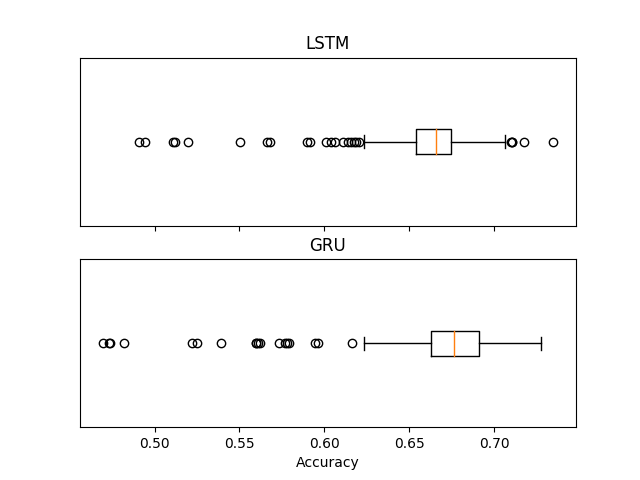
\includegraphics[width=0.45\textwidth]{Figures/lstm_gru_plot.png}
      \caption{Comparing the performance of LSTM and GRU cells over all
        parameter measurements}
      \label{fig:lstm_gru}
    \end{figure}

    Figure \ref{fig:lstm_gru} compares the performance of LSTM and GRU cells
    over all measurements. The GRU cell achieved a higher
    median, lower and upper quartile accuracy than the LSTM cell. However, including
    outliers, the GRU cell was less consistent: achieving the lowest accuracy
    single result. The highest accuracy was an LSTM cell but this was only by a
    small margin.

    \begin{figure}[ht]
      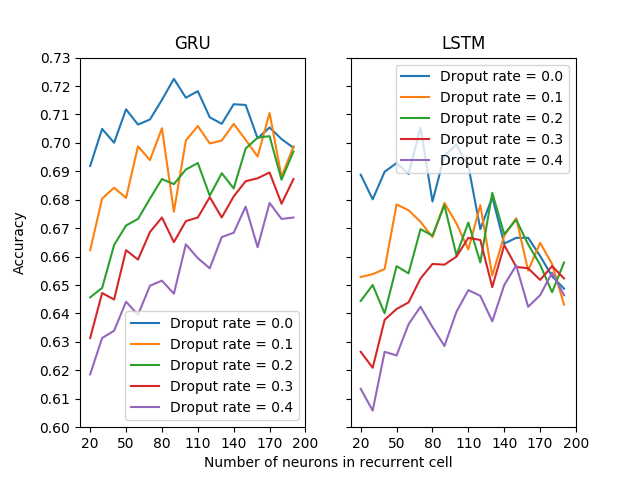
\includegraphics[width=0.45\textwidth]{Figures/n_neurons_plot-0-0001.png}
      \caption{Using a learning rate of 0.0001: the relationship between the number of neurons in the recurrent
        cell to classification accuracy for GRU and LSTM at each dropout rate.}
      \label{fig:learn_rate_0.0001}
    \end{figure}

    Figure \ref{fig:learn_rate_0.0001} shows the results for training using a
    learning rate of 0.0001. At this learning rate the GRU saw slight improvements in
    accuracy with an increasing number of neurons up to 100, after which
    accuracy declined. This decline was likely due to minor overfitting of the
    training set. However, even the lowest dropout rates only approached
    performance on par with no dropout for the largest numbers of neurons
    tested. For most of the data, there was a clear accuracy reduction from an
    increase in the dropout rate.

    The LSTM cell performed much less well than GRU at this learning rate, with
    classification accuracy quickly declining for numbers of neurons higher than
    110. The dropout rate was similarly detrimental as for the GRU at
    small numbers of neurons. As performance degraded at higher numbers of
    neurons, moderate dropout rates (up to 0.2) out-performed the network without
    dropout. This suggests more severe overfitting than for the GRU cell,
    perhaps because LSTM is a more complex construction. 

    \begin{figure}[ht]
      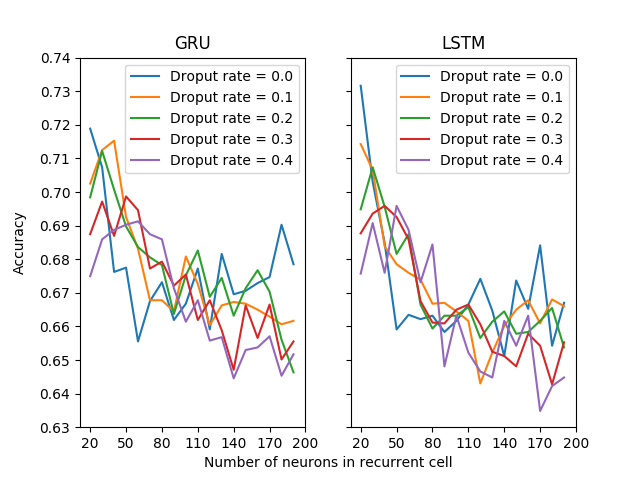
\includegraphics[width=0.45\textwidth]{Figures/n_neurons_plot-0-001.png}
      \caption{Using a learning rate of 0.001: the relationship between the number of neurons in the recurrent
        cell to classification accuracy for GRU and LSTM at each dropout rate.}
      \label{fig:learn_rate_0.001}
    \end{figure}

    Figure \ref{fig:learn_rate_0.001} shows results for a higher learning rate
    of 0.001. At this higher learning rate there was a clear performance
    degradation as the number of neurons was increased, particularly up to 100
    neurons. The results are also far more chaotic, with measurements spiking up
    and down. In further tests it was confirmed that there was a higher variance in
    the results at this learning rate compared to the previous. Results at a
    further increased learning rate of 0.01 varied so much as to be
    un-reproducible. This suggests that a learning rate of 0.001 was too high to
    capture the features of this optimisation problem, with the issue worsening
    as neurons are added: increasing the complexity of the fitness landscape.
    This higher learning rate achieved the highest accuracies in the test when
    using smaller neurons. This may indicate that the smaller 0.0001 learning rate grid
    search had not trained over sufficient epochs before stopping - giving the
    higher learning rate the upper hand in the simpler learning problems.

    Dropout rates seem to have had much less of an effect at this higher
    learning rate, however, the highest results were still mostly obtained by
    the lower dropout rates. The cell type also seemed to have much less of an
    affect. Perhaps the problems training with this higher learning rate also
    reduced overfitting.

    Following from these observations from the grid search, recursive neural
    networks were trained using a learning rate of 0.0001 over 10 times as many
    epochs using a variety of lower dropout rates. These models did eventually
    overfit much more severely - achieving training set accuracy of around 90\%
    but only 70\% test accuracy and log-loss of 1.09. Small changes in the
    dropout rate had very little effect upon the performance of the RNN. The
    confusion matrix is given in table \ref{tab:rnn_res}

\begin{table}[h]
\centering
\begin{tabular}{m{1cm}|m{1cm}|m{1cm}|m{1cm}|m{0cm}}
\multicolumn{1}{m{1cm}}{} & \multicolumn{1}{m{1cm}}{EAP} & \multicolumn{1}{m{1cm}}{HPL} & \multicolumn{1}{m{1cm}}{MWS} &\\[5pt]
\cline{2-4}
EAP & 721 & 261 & 120 & \\[5pt]
\cline{2-4}
HPL & 163 & 1218 & 219 & \\[5pt]
\cline{2-4}
MWS & 120 & 311 & 783 & \\[5pt]
\cline{2-4}
\end{tabular}
\caption{Final results for RNN\\Loss 1.09 Accuracy: 70\% }
\label{tab:rnn_res}
\end{table}


    \subsection{Ensemble}
    \label{sec:ensemble}

    It was expected that the windowed neural network and the bag of words neural
    network would be reasonably uncorrelated because they used such different
    input features. To take advantage of this they were combined into an
    ensemble using a single densely connected perceptron layer with sigmoid
    activation to combine their weights. However, when tested, this ensemble
    performed the same as the bag of words neural network, presumably having
    learnt to reproduce its output.

\subsection{KPCA}
\label{sec:kpca}
  
